
\begin{frame}{Simulation}{Map}
  \begin{block}{Topographic map used in the simulation}
  	\begin{itemize}
	 	\item LOS Distance
	  	\item Coverage Map
	\end{itemize}
	\begin{figure}
    	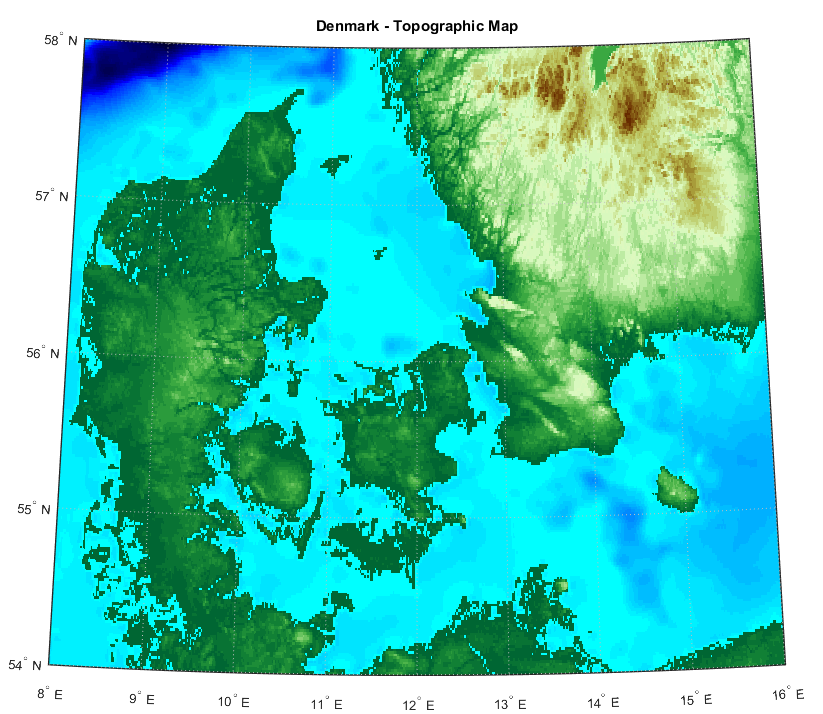
\includegraphics[scale=0.28]{../report/figures/dk_map.png}
    \end{figure}
  \end{block}
\end{frame}

\begin{frame}{Simulation}{LOS Distance}
  \begin{figure}
    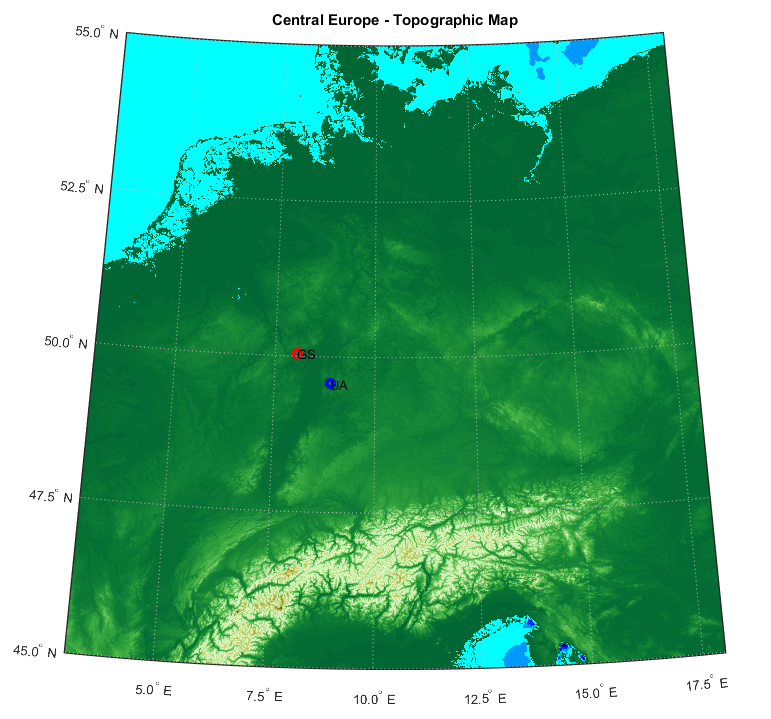
\includegraphics[scale=0.25]{../report/figures/gs_ua_map.png}
  \end{figure}
  \begin{block}{Parameters taken into account}
	\begin{itemize}
	 	\item Terrain elevation
	  	\item Curvature of the Earth
	  	\item Altitude of UA and GS
	\end{itemize}
  \end{block}
\end{frame}

\begin{frame}{Simulation}{LOS Distance between UA and GS} 
  	\begin{figure}
        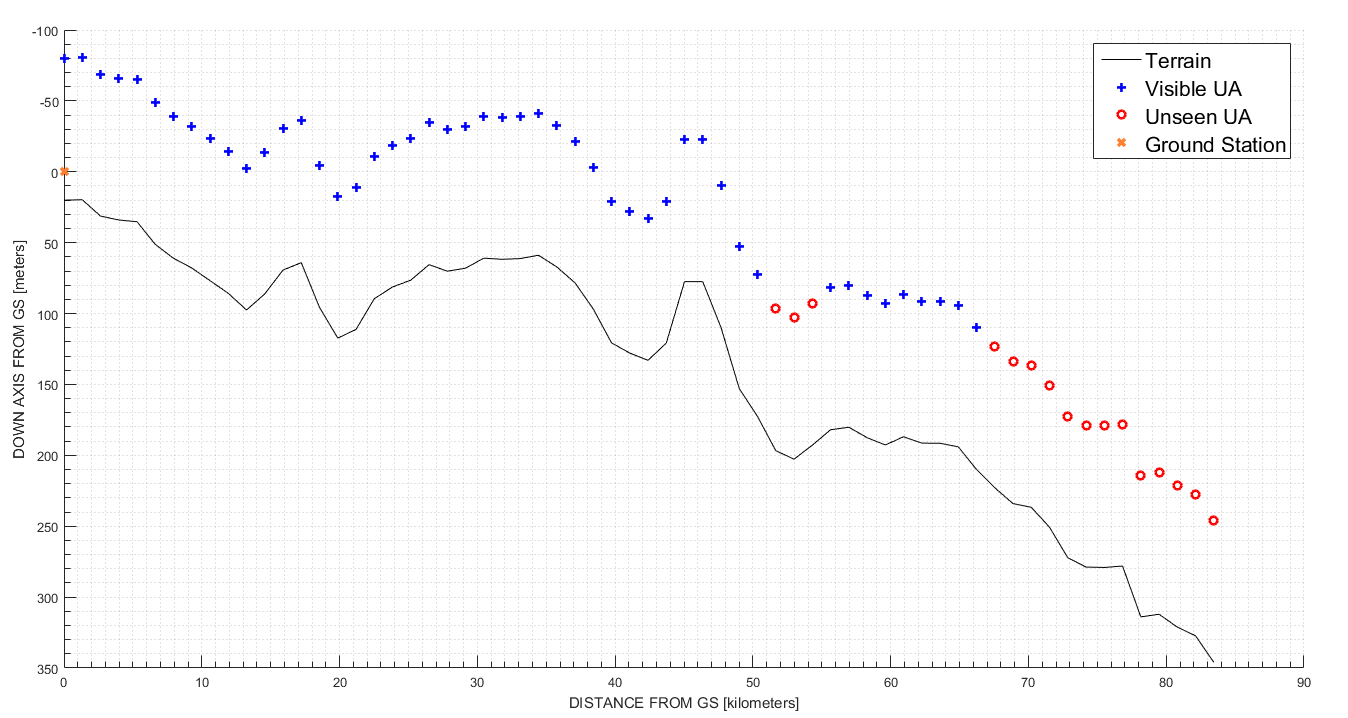
\includegraphics[scale=0.29]{../report/figures/los_2points.png}
    \end{figure}
\end{frame}

\begin{frame}{Simulation}{LOS Coverage Map}
  \begin{block}{Plot LOS area around GS}
	\begin{figure}
    	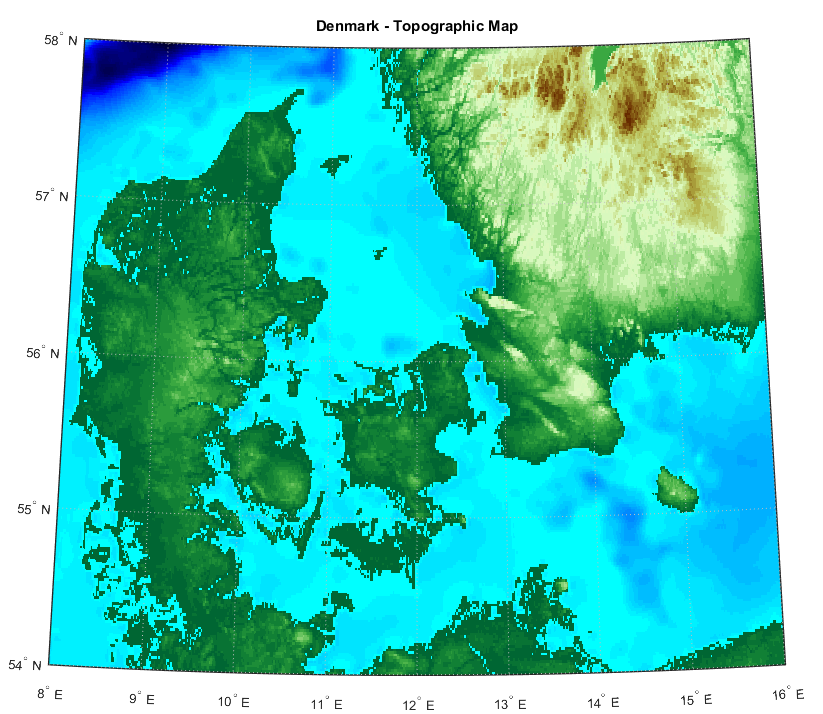
\includegraphics[scale=0.33]{../report/figures/dk_map.png}
    \end{figure}
  \end{block}
\end{frame}

\begin{frame}{Simulation}{LOS Coverage Map} 
  	\begin{figure}
        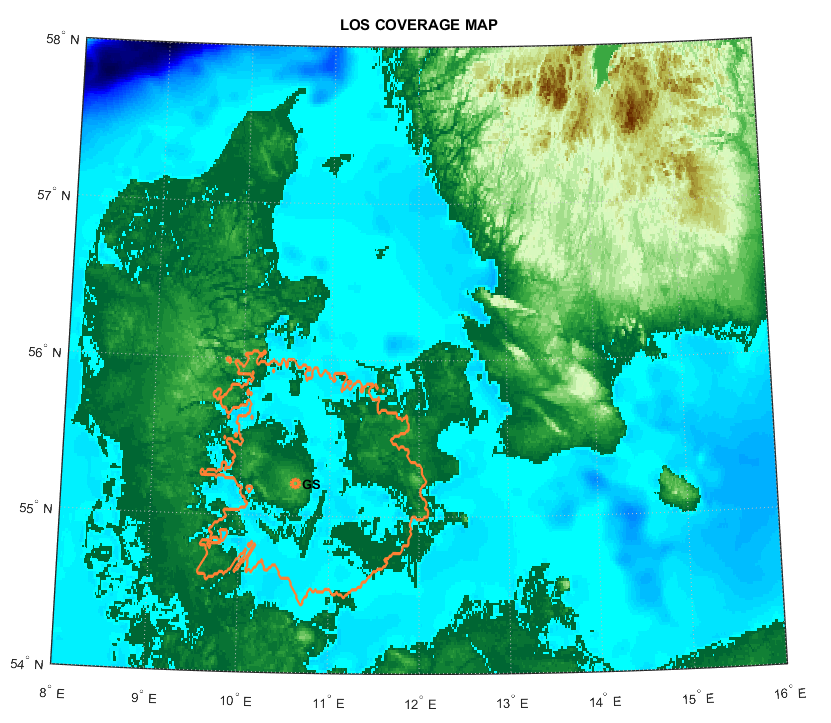
\includegraphics[scale=0.40]{../report/figures/los_odense.png}
    \end{figure}
\end{frame}

\begin{frame}{Simulation}{2D UAS}
	\begin{block}{2D UAS Block Diagram}
		\begin{itemize}
		  	\item Cartesian system
		  	\item 1 DoF - azimuth angle ($\theta$)
		  	\item Compute optimal azimuth angle for UA and GS 
		\end{itemize}

		\begin{figure}
	        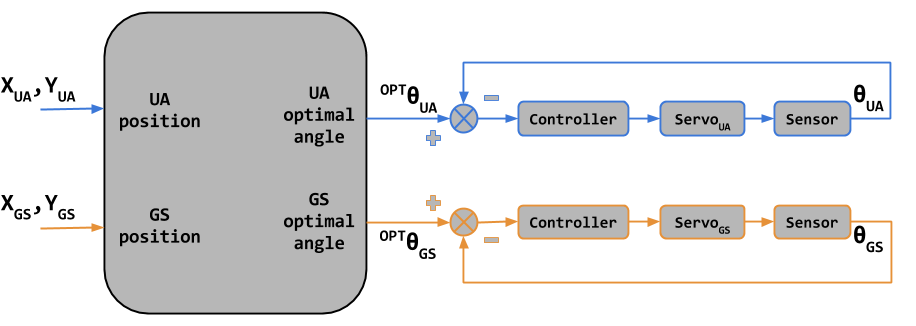
\includegraphics[scale=0.32]{figures/2D_system.png}
	    \end{figure}
    \end{block}
\end{frame}

\begin{frame}{Simulation}{3D UAS}
  \begin{block}{3D UAS Block Diagram}
	\begin{itemize}
	  	\item Realistic Earth model - WGS84
	  	\item Relief of Earth's surface 
	  	\item Real GPS position: latitude, longitude and altitude
	\end{itemize}

	\begin{figure}
		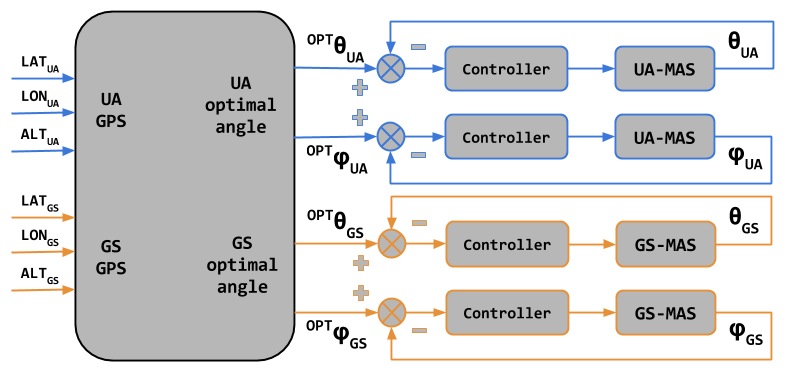
\includegraphics[scale=0.33]{figures/3D_system.png}
	\end{figure}
  \end{block}
\end{frame}

% \begin{frame}{Simulation}{3D UAS}
%   \begin{block}{Simulation steps}
% 	  \begin{enumerate}
% 	  	\item Aquire GPS position of GS and UA 
% 	  	\item Compute optimal angles and error signal 
% 	  	\item Input error signal in the controller
% 	  	\item Limit output signal from controller using the saturation box
% 	  	\item Input controller signal to the servomotor
% 	  	\item Feedback the output angle in the optimal angle block
% 	  \end{enumerate}
%   \end{block}
% \end{frame}

\begin{frame}{Simulation}{3D UAS}
  \begin{block}{Simulation assumptions}
	  \begin{itemize}
	  	\item Same antenna parameters for GS and UA
	  	\item Same MAS model for GS and UA
	  	\item Saturation box threshold set from $-5V$ to $+5V$
	  	\item Noise modelled as Gaussian White Noise of power $10^{-4}$
	  	\item Azimuth and elevation angles start at 0 degrees
	  \end{itemize}
  \end{block}
\end{frame}